\chapter{Quantum singular value transformation}\label{chap:qsvt}

In \cref{chap:hermfunc}, we have found that using qubitization, we can effectively block encode the Chebyshev matrix polynomial $T_k(A)$ for a Hermitian matrix $A$.
Combined with LCU, we can construct a block encoding of any matrix polynomial of $A$.
The process is greatly simplified using QSP and QET, which allows the implementation a general class of matrix functions for Hermitian matrices.

In this section, we generalize the results of qubitization and QET to general non-Hermitian matrices. 
This is called the quantum singular value transformation (QSVT).
Throughout the chapter we assume $A\in\CC^{N\times N}$ is a square matrix.
QSVT is applicable to non-square matrices as well, and we will omit the discussions here.




\section{Generalized matrix functions}


For a square matrix $A \in \mathbb{C}^{N \times N}$, where for simplicity we assume $N=2^n$ for some positive integer $n$, the singular value decomposition (SVD) of the normalized matrix $A$ can be written as
\begin{equation}
A=W\Sigma V^{\dag},
\label{eqn:A_SVD}
\end{equation}
or equivalently
\begin{equation}
A\left|v_{i}\right\rangle= \sigma_{i}\left|w_{i}\right\rangle, \quad A^{\dagger}\left|w_{i}\right\rangle= \sigma_{i}\left|v_{i}\right\rangle, \quad i\in [N].
\label{eqn:A_svd_component}
\end{equation}
We may apply a function $f(\cdot)$ on its singular values and define the generalized matrix function \cite{HawkinsBen-Israel1973,ArrigoBenziFenu2016} as below.

\begin{defn}[Generalized matrix function {\cite[Definition 4]{ArrigoBenziFenu2016}}]
\label{def:gen_matrix_function}
Given $A\in\CC^{N\times N}$ with singular value decomposition \cref{eqn:A_SVD}, and let $f: \mathbb{R} \rightarrow \mathbb{\CC}$ be a scalar function such that $f\left(\sigma_{i}\right)$ is defined for all $i\in[N]$. The generalized matrix function is defined as
\begin{equation}
f^{\diamond}(A):=Wf(\Sigma)V^{\dag},
\label{eqn:gen_matrix_function}
\end{equation}
where 
$$
f\left(\Sigma\right)=\operatorname{diag}\left(f\left(\sigma_{0}\right), f\left(\sigma_{1}\right), \ldots, f\left(\sigma_{N-1}\right)\right).
$$
\end{defn}

Given the form in \cref{eqn:A_svd_component}, we also define two other types of generalized matrix functions.

\begin{defn}Under the conditions in \cref{def:gen_matrix_function}, the left and right generalized matrix function are defined respectively as
\begin{equation}
f^{\triangleleft}(A):=Wf(\Sigma)W^{\dag}, \quad 
f^{\triangleright}(A):=Vf(\Sigma)V^{\dag}.
\label{eqn:gen_matrix_function_lr}
\end{equation}
\label{def:gen_matrix_function_lr}
\end{defn}

Here the left and right pointing triangles reflects that the transformation only keeps the left and right singular vectors, respectively.
For a given $A$, somewhat confusingly, in the discussion below, the transformation $f^{\triangleright}(A),f^{\triangleleft}(A),f^{\diamond}(A)$ will all be referred to as \emph{singular value transformations}.
In particular, QSVT mainly concerns $f^{\triangleright}(A),f^{\diamond}(A)$.

\begin{prop}
The following relations hold:
\begin{equation}
f^{\diamond}(A^{\dag})=(f^{\diamond}(A))^{\dag}, \quad f^{\triangleright}(A)=f^{\triangleleft}(A^{\dag}),
\end{equation}
and
\begin{equation}
f^{\triangleright}(A)=f^{\diamond}(\sqrt{A^{\dag}A})=f(\sqrt{A^{\dag}A}), \quad
f^{\triangleleft}(A)=f^{\diamond}(\sqrt{A A^{\dag}})=f(\sqrt{A A^{\dag}}). \end{equation}
\label{prop:gen_mat_func_relation}
\end{prop}
\begin{proof}
Just note that $A^{\dag}A=V\Sigma^2 V^{\dag}$, we have $\sqrt{A^{\dag}A}=V\Sigma V^{\dag}$. So the eigenvalue and singular value decomposition coincide for both $\sqrt{A^{\dag}A}$ and $\sqrt{A A^{\dag}}$.
\end{proof}

WLOG we assume access to $U_A\in\BE_{1,m}(A)$, so that the singular values of $A$ are in $[0,1]$, i.e.,
\begin{equation}
0\le \sigma_i \le 1, \quad i\in[N].
\end{equation}

\section{Qubitization of general matrices}\label{sec:qubitize_general}

In \cref{sec:qubitize_genbe} we have observed that when $A$ is a Hermitian matrix, the qubitization procedure introduces two different subspaces $\mc{H}_i$ and $\mc{H}_i'$ associated with each eigenvector $\ket{v_i}$.
In particular, $U_A$ maps  $\mc{H}_i$ to $\mc{H}_i'$, and $U_A^{\dag}$ maps $\mc{H}_i'$ to $\mc{H}_i$. 
Furthermore, both $\mc{H}_i$ and $\mc{H}_i'$ are the invariant subspaces of the projection operator $\Pi$.
Therefore $\mc{H}_i$ is an invariant subspace of $U_A^{\dag} f(\Pi) U_A$ for any function $f$. 
Much of the same structure can be carried out to the quantum singular value transformation.
The only difference is that the qubitization is now defined with respect to the singular vectors. 
The procedure below almost entirely parallelizes that of \cref{sec:qubitize_genbe}, except that we need to work with the singular value decomposition instead of the eigenvalue decomposition.

Start from the SVD in \cref{eqn:A_svd_component}, we apply $U_A$ to $\ket{0^m}\ket{v_i}$ and obtain 
\begin{equation}
U_A\ket{0^m}\ket{v_i}=\sigma_i\ket{0^m}\ket{w_i}+\sqrt{1-\sigma_i^2}\ket{\perp_i'},
\label{eqn:UA_apply_vi_2_qsvt}
\end{equation}
where $\ket{\perp_i'}$ is a normalized state satisfying $\Pi\ket{\perp_i'}=0$.

Since $U_A$ block encodes a matrix $A$, we have
\begin{equation}
U_A^{\dag}=\begin{pmatrix}
{A}^{\dag} & {*} \\
{*} & {*}
\end{pmatrix},
\end{equation}
which implies that there exists another normalized state $\ket{\perp_i}$ satisfying $\Pi\ket{\perp_i}=0$ and
\begin{equation}
U^{\dag}_A\ket{0^m}\ket{w_i}=\sigma_i\ket{0^m}\ket{v_i}+\sqrt{1-\sigma_i^2}\ket{\perp_i}.
\label{eqn:Udag_apply_vi_qsvt}
\end{equation}
Now apply $U_A$ to both sides of \cref{eqn:Udag_apply_vi_qsvt}, we obtain
\begin{equation}
\ket{0^m}\ket{w_i}=\sigma^2_i\ket{0^m}\ket{w_i}+\sigma_i\sqrt{1-\sigma_i^2}\ket{\perp_i'} +\sqrt{1-\sigma_i^2}U_A\ket{\perp_i},
\end{equation}
which gives
\begin{equation}
U_A\ket{\perp_i}=\sqrt{1-\sigma_i^2}\ket{0^m}\ket{w_i}-\sigma_i\ket{\perp_i'}.
\label{eqn:UA_apply_perpi_2_qsvt}
\end{equation}
Define
\begin{equation}
\mc{B}_i=\{\ket{0^m}\ket{v_i},\ket{\perp_i}\}, \quad \mc{B}'_i=\{\ket{0^m}\ket{w_i},\ket{\perp_i'}\},
\end{equation}
and the associated two-dimensional subspaces $\mc{H}_i=\opr{span}{B_i}, \mc{H}'_i=\opr{span}{B_i'}$, we find that $U_A$ maps $\mc{H}_i$ to $\mc{H}_i'$.
Correspondingly $U_A^{\dag}$ maps $\mc{H}_i'$ to $\mc{H}_i$.

Then \cref{eqn:UA_apply_vi_2_qsvt,eqn:UA_apply_perpi_2_qsvt} give the matrix representation
\begin{equation}
[U_A]_{\mc{B}_i}^{\mc{B}_i'}=\begin{pmatrix}
\sigma_i & \sqrt{1-\sigma_i^2}\\
\sqrt{1-\sigma_i^2} & -\sigma_i
\end{pmatrix}.
\end{equation}
Similar calculation shows that
\begin{equation}
[U^{\dag}_A]_{\mc{B}_i'}^{\mc{B}_i}=\begin{pmatrix}
\sigma_i & \sqrt{1-\sigma_i^2}\\
\sqrt{1-\sigma_i^2} & -\sigma_i
\end{pmatrix}.
\end{equation}
Meanwhile both $\mc{H}_i$ and $\mc{H}_i'$ are the invariant subspaces of the projector $\Pi$, with matrix representation
\begin{equation}
[\Pi]_{\mc{B}_i}=[\Pi]_{\mc{B}_i'}=\begin{pmatrix}
1 & 0 \\
0 & 0
\end{pmatrix}.
\end{equation}
Therefore
\begin{equation}
[Z_\Pi]_{\mc{B}_i}=[Z_\Pi]_{\mc{B}_i'}=\begin{pmatrix}
1 & 0 \\
0 & -1
\end{pmatrix}.
\end{equation}
Hence $\mc{H}_i$ is an invariant subspace of $\wt{O}=U_A^{\dag}Z_{\Pi}U_A Z_{\Pi}$, with matrix representation
\begin{equation}
[\wt{O}]_{\mc{B}_i}=\begin{pmatrix}
\sigma_i & -\sqrt{1-\sigma_i^2}\\
\sqrt{1-\sigma_i^2} & \sigma_i
\end{pmatrix}^2.
\end{equation}
Repeating $k$ times, we have
\begin{equation}
\begin{split}
[\wt{O}^k]_{\mc{B}_i}=&(U_A^{\dag}Z_{\Pi}U_A Z_{\Pi})^{k}=\begin{pmatrix}
\sigma_i & -\sqrt{1-\sigma_i^2}\\
\sqrt{1-\sigma_i^2} & \sigma_i
\end{pmatrix}^{2k}\\
=&\begin{pmatrix}
T_{2k}(\sigma_i) & -\sqrt{1-\sigma_i^2}U_{2k-1}(\sigma_i)\\
\sqrt{1-\sigma_i^2}U_{2k-1}(\sigma_i) & T_{2k}(\sigma_i)
\end{pmatrix}.
\end{split}
\end{equation}
In other words, 
\begin{equation}
\wt{O}^k=\begin{pmatrix}
\sum_{i} v_i T_{2k}(\sigma_i) v_i^{\dag} & *\\
* & *
\end{pmatrix}
=\begin{pmatrix}
T^{\triangleright}_{2k}(A) & *\\
* & *
\end{pmatrix}.
\end{equation}
Therefore the circuit $(U_A^{\dag}Z_{\Pi}U_A Z_{\Pi})^{k}$ gives $(1,m)$-block-encoding of $T_{2k}^{\triangleright}(A)$.

Similarly,
\begin{equation}
[U_A Z_{\Pi}(U_A^{\dag}Z_{\Pi}U_A Z_{\Pi})^{k}]_{\mc{B}_i}^{\mc{B}_{i}'}=\begin{pmatrix}
T_{2k+1}(\sigma_i) & -\sqrt{1-\sigma_i^2}U_{2k}(\sigma_i)\\
\sqrt{1-\sigma_i^2}U_{2k}(\sigma_i) & T_{2k+1}(\sigma_i)
\end{pmatrix}.
\end{equation}
In other words, \begin{equation}
U_A Z_{\Pi}(U_A^{\dag}Z_{\Pi}U_A Z_{\Pi})^{k}=\begin{pmatrix}
\sum_{i} w_i T_{2k+1}(\sigma_i) v_i^{\dag} & *\\
* & *
\end{pmatrix}
=\begin{pmatrix}
T^{\diamond}_{2k+1}(A) & *\\
* & *
\end{pmatrix}.
\end{equation}
Therefore the circuit $U_A Z_{\Pi}(U_A^{\dag}Z_{\Pi}U_A Z_{\Pi})^{k}$ gives $(1,m)$-block-encoding of $T_{2k+1}^{\diamond}(A)$. 

\begin{rem}
By approximating any continuous function $f$ using polynomials, and using the LCU lemma, we can approximately evaluate $f^{\diamond}(A)$ for any odd function $f$, and $f^{\triangleright}(A)$ for any even function $f$.
This may seem somewhat restrictive.
However, note that all singular values are non-negative.
Hence when performing the polynomial approximation, if we are interested in $f^{\diamond}(A)$, we can always use first perform a polynomial approximation of an \emph{odd extension} of $f$, i.e.,
\begin{equation}
g(x)=\begin{cases}
f(x), & x>0,\\
0, & x=0, \\
-f(-x), & x<0,
\end{cases}
\end{equation}
and then evaluate $g^{\diamond}(A)$.
Similarly, if we are interested in $f^{\triangleright}(A)$ for a general $f$, we can perform polynomial approximation to its \emph{even extension}
\begin{equation}
g(x)=\begin{cases}
f(x), & x\ge0,\\
f(-x), & x<0,
\end{cases}
\end{equation}
and evaluate $g^{\triangleright}(A)$.
\end{rem}

\section{Quantum singular value transformation}\label{sec:qsvt}

\subsection{Quantum circuit}

Due to the close relation between eigenvalue and singular value transformation in terms of Chebyshev polynomials and qubitization in \cref{sec:qubitize_general}, we can obtain the QSVT circuit easily following the discussion in \cref{sec:qsp}.


First, there are no changes to the scalar case of QSP (in terms of SU(2) matrices), and in particular \cref{thm:qsp} and \cref{thm:qsp_real}.

For the matrix case, when $d$ is even,
\begin{equation}
U_{\Phi}=(-\I)^d e^{\I \wt{\phi}_0 Z_{\Pi}} 
\prod_{j=1}^{d/2}\left[ U^{\dag}_A e^{\I \wt{\phi}_{2j-1} Z_{\Pi}}U_A e^{\I \wt{\phi}_{2j} Z_{\Pi}} \right]
\end{equation}
gives a $(1,m+1)$-block-encoding of $P^{\triangleright}(A)$ for some even polynomial $P\in\CC[x]$.

When $d$ is odd, 
\begin{equation}
U_{\Phi}=(-\I)^d e^{\I \wt{\phi}_0 Z_{\Pi}} (U_A e^{\I \wt{\phi}_{1} Z_{\Pi}})
\prod_{j=1}^{(d-1)/2}\left[ U^{\dag}_A e^{\I \wt{\phi}_{2j} Z_{\Pi}}U_A e^{\I \wt{\phi}_{2j+1} Z_{\Pi}} \right]
\end{equation}
gives a $(1,m+1)$-block-encoding of $P^{\diamond}(A)$ for some odd polynomial $P\in\CC[x]$.

The quantum circuit is exactly the same as that in \cref{fig:qet_circuit_general}.
The phase factors can be adjusted so that all polynomials $P$ satisfying the conditions in \cref{thm:qsp} can be exactly represented.
If we are only interested in some real polynomial $P_{\Re}\in\RR[x]$ and $P_{\Re}^{\diamond}(A)$ (odd) and $P^{\triangleright}(A)$ (even), we can use \cref{thm:qsp_real} and the circuit in \cref{fig:qsvt_circuit_real} (which is simply a combination of \cref{fig:qet_circuit_general_real,fig:qet_circuit_general}) to implement its $(1,m+1)$-block-encoding.
We have the following theorem.
Since the conditions of QSP representation for real polynomials is simple to satisfy and is also most useful in practice, we only state the case with real polynomials.

\begin{thm}[Quantum singular value transformation with real polynomials]
Let $A\in\CC^{N\times N}$ be encoded by its $(1,m)$-block-encoding $U_A$.
Given a polynomial $P_{\Re}(x)\in\RR[x]$ of degree $d$ satisfying the conditions in \cref{thm:qsp_real}, we can find a sequence of phase factors $\Phi\in\RR^{d+1}$, so that the circuit in \cref{fig:qsvt_circuit_real} denoted by $U_{\Phi}$ implements a $(1,m+1)$-block-encoding of $P^{\diamond}_{\Re}(A)$ if $d$ is odd, and of $P^{\triangleright}_{\Re}(A)$ if $d$ is even.
$U_{\Phi}$ uses $U_A,U_A^{\dag}$, m-qubit controlled NOT, and single qubit rotation gates for $\Or(d)$ times.
\label{thm:qsvt_real}
\end{thm}


\begin{figure}[H]
  \begin{quantikz}
    \lstick{$\ket{0}$} & \gate{H}& \gate[2]{\opr{CR}_{\wt{\phi}_d}} & \qw & \gate[2]{\opr{CR}_{\wt{\phi}_{d-1}}} & \qw & \qw \raisebox{0em}{$\cdots$}&\qw& \gate[2]{\opr{CR}_{\wt{\phi}_0}}&\qw&\gate{H} &\qw\\
    \lstick{$\ket{0^m}$} &\qw&\qw& \gate[2]{U_A} &  \qw  & \gate[2]{U^{\dag}_A} &\qw\raisebox{0em}{$\cdots$} &\gate[2]{U_A}&\qw&\qw&\qw&\qw\\
    \lstick{$\ket{\psi}$}&\qw& \qw& \qw& \qw& \qw& \qw\raisebox{0em}{$\cdots$}&\qw&\qw&\qw&\qw&\qw
  \end{quantikz}
  \caption{Circuit of quantum singular value transformation to construct $U_{P^{\diamond}_{\Re}}\in\BE_{1,m+1}(P^{\diamond}_{\Re}(A))$, using $U_A\in\BE_{1,m}(A)$.
  Here $U_A,U_A^{\dag}$ should be applied alternately.  When $d$ is even, the last $U_A$ gate should be replaced $U_A^{\dag}$, and the circuit constructs $U_{P^{\triangleright}_{\Re}}\in\BE_{1,m+1}(P^{\triangleright}_{\Re}(A))$. This is simply a combination of \cref{fig:qet_circuit_general_real,fig:qet_circuit_general}.}
  \label{fig:qsvt_circuit_real}
\end{figure}


\subsection{QSVT applied to Hermitian matrices}

When $A$ is a Hermitian matrix, the quantum circuit for QET and QSVT are the same.
This means that the eigenvalue transformation and the singular value transformation are merely two different perspectives of the same object.

For a Hermitian matrix $A$, the eigenvalue decomposition and the singular value decomposition are connected as
\begin{equation}
A=\sum_{i} \ket{v_i}\lambda_i \bra{v_i}=\sum_{i} \ket{\opr{sgn}(\lambda_i)v_i} \abs{\lambda_i} \bra{v_i}:=\sum_{i} \ket{w_i} \sigma_i \bra{v_i}.
\end{equation}
Here 
\begin{equation}
\ket{w_i}=\ket{\opr{sgn}(\lambda_i)v_i}, \quad \sigma_i=\abs{\lambda_i}.
\end{equation}
So if $P\in\CC[x]$ is an even polynomial,
\begin{equation}
P(A)=\sum_{i} \ket{v_i}P(\lambda_i)\bra{v_i}=\sum_{i} \ket{v_i}P(\abs{\lambda_i})\bra{v_i}=P^{\triangleright}(A).
\end{equation}
Similarly, if $P\in\CC[x]$ is an odd polynomial, then
\begin{equation}
P(A)=\sum_{i} \ket{v_i}P(\lambda_i)\bra{v_i}=\sum_{i} \ket{\opr{sgn}(\lambda_i)v_i}P(\abs{\lambda_i})\bra{v_i}=P^{\diamond}(A).
\end{equation}
These relations indeed verify that the eigenvalue decomposition and singular value decomposition are indeed the same when $P$ has a definite parity.
When the parity of $P$ is indefinite, the two objects are in general not the same, and in particular cannot be directly implemented using the QET circuit. 

\subsection{QSVT and matrix dilation}

For general matrices, we have seen in the context of solving linear equations in \cref{sec:HHL} that the matrix dilation method in \cref{eqn:dilation_hermitian} can be used to convert the non-Hermitian problem to a Hermitian problem.
Here we study the relation between QSP applied to the dilated Hermitian matrix, and QSVT for the general matrix.

Recall the definition of the dilated Hermitian matrix 
\begin{equation}
\label{eqn:dilation_trick}
    \wt{A}= \begin{bmatrix} 0 & A^\dagger\\ A & 0 \end{bmatrix}.
\end{equation}
When $A$ is given by its block encoding $U_A\in\BE_{1,m}(A)$, the dilated Hermitian matrix $\wt{A}$ can be obtained with one ancilla qubit through $U_{\wt{A}}=\ket{0}\bra{1}\otimes U_A + \ket{1}\bra{0}\otimes U_A^\dagger$, i.e., $U_{\wt{A}}\in\BE_{1,m+1}(\wt{A})$. Note that this requires the controlled version of $U_A,U_A^{\dag}$. 

From the SVD in \cref{eqn:A_svd_component}, we can construct 
\begin{equation}
\ket{z^{\pm}_i}=\frac{1}{\sqrt{2}}(\ket{0}\ket{v_i}\pm\ket{1}\ket{w_i}).
\end{equation}
Direct calculation shows
\begin{equation}
\wt{A}\ket{z^{\pm}_i}=\pm \sigma_i \ket{z^{\pm}_i},
\end{equation}
i.e., $\{\ket{z^{\pm}_i}\}$ are all the eigenvectors of $\wt{A}$.

For an arbitrary polynomial $f\in\CC[x]$, the matrix function applied to $\wt{A}$ can be computed as
\begin{equation}
\begin{split}
f(\wt{A})&= \sum_{i} \ket{z^{+}_i} f(\sigma_i) \bra{z^{+}_i}+
\ket{z^{-}_i} f(-\sigma_i) \bra{z^{-}_i}\\
&=\sum_{i} \begin{pmatrix}
\ket{v_i} f_{\mathrm{even}}(\sigma_k)\bra{v_i} & \ket{v_i} f_{\mathrm{odd}}(\sigma_k)\bra{w_i}\\
\ket{w_i} f_{\mathrm{odd}}(\sigma_k)\bra{v_i} & \ket{w_i} f_{\mathrm{even}}(\sigma_k)\bra{w_i}\\
\end{pmatrix}\\
&=\begin{pmatrix}
f^{\triangleright}_{\mathrm{even}}(A) & f^{\diamond}_{\mathrm{odd}}(A^{\dag})\\
f^{\diamond}_{\mathrm{odd}}(A)& f^{\triangleleft}_{\mathrm{even}}(A)
\end{pmatrix}.
\end{split}
\end{equation}
Here 
\begin{equation}
f_{\mathrm{even}}(x)=\frac12(f(x)+f(-x)), \quad f_{\mathrm{odd}}(x)=\frac12(f(x)-f(-x)).
\end{equation}
Therefore applying the QSP to the dilated matrix $\wt{A}$ automatically implements QSVT of $A$ using polynomials of even and odd parities.

In particular, if $f$ is an even function, then 
\begin{equation}
f(\wt{A})\ket{0}\ket{\psi}=\ket{0}f^{\triangleright}(A)\ket{\psi},
\end{equation}
i.e., measuring the signal qubit we obtain $0$ with certainty, and the system register is $f^{\triangleright}_{\mathrm{even}}(A)\ket{\psi}$.
Similarly, if $f$ is odd, then
\begin{equation}
f(\wt{A})\ket{0}\ket{\psi}=\ket{1}f^{\diamond}(A)\ket{\psi},
\end{equation}
i.e., measuring the signal qubit we obtain $1$ with certainty.


\section{Application: Solve linear systems of equations}\label{sec:appqsvt_qlsp}

In this section, we revisit the problem of solving linear systems of equations $Ax=b$. With QSVT we can solve QLSP for general matrices without the need of dilating the matrix into a Hermitian matrix.
Assume $A=W\Sigma V^{\dag}$ is invertible, i.e., $\forall i, \Sigma_{ii}>0$, then
\begin{equation}
A^{-1}=V \Sigma^{-1} W^\dagger=f^{\diamond}(A^\dagger),
\label{eqn:ainv_qsvt}
\end{equation}
where $f(x)=x^{-1}$ is an odd function. 


WLOG assume $A$ can be accessed by $U_A\in\BE_{1,m}(A)$. For simplicity we also assume $\norm{A}=1$ (though in general $\norm{A}\le \alpha=1$, and we may not always be able to set $\norm{A}=1$).
Let $\kappa$ be the condition number of $A$, then the singular values of $A$ are contained in the interval $[\delta,1]$, with $\delta =\kappa^{-1}$.

Note that $f(\cdot)$  is not bounded by 1 and in particular singular at $x=0$. Therefore instead of approximating $f$ on the whole interval $[-1,1]$ we consider an odd polynomial $p(x)$ such that
\begin{equation}
\left|p(x)-\frac{\delta}{\beta x}\right|\leq \epsilon',\quad \forall x\in [-1,-\delta]\cup[\delta,1].
\end{equation}
The $\beta$ factor is chosen arbitrarily so that $|p(x)|\leq 1$ for all $x\in[-1,1]$ to satisfy the requirement of the condition (2) in \cref{thm:qsp_real}. For instance, we may choose $\beta=4/3$. The precision parameter $\epsilon'$ will be chosen later.
The degree of the odd polynomial can be chosen to be $\Or(\frac{1}{\delta}\log(\frac{1}{\epsilon'}))$ is guaranteed by e.g. \cite[Corollary 69]{GilyenSuLowEtAl2018}.
This construction is not explicit (see an explicit construction in~\cite{ChildsKothariSomma2017}).
\cref{fig:qsp_inv_deg81} gives a concrete construction of an odd polynomial obtained via numerical optimization, and the phase factors are obtained via QSPPACK.


\begin{figure}[H]
\begin{center}
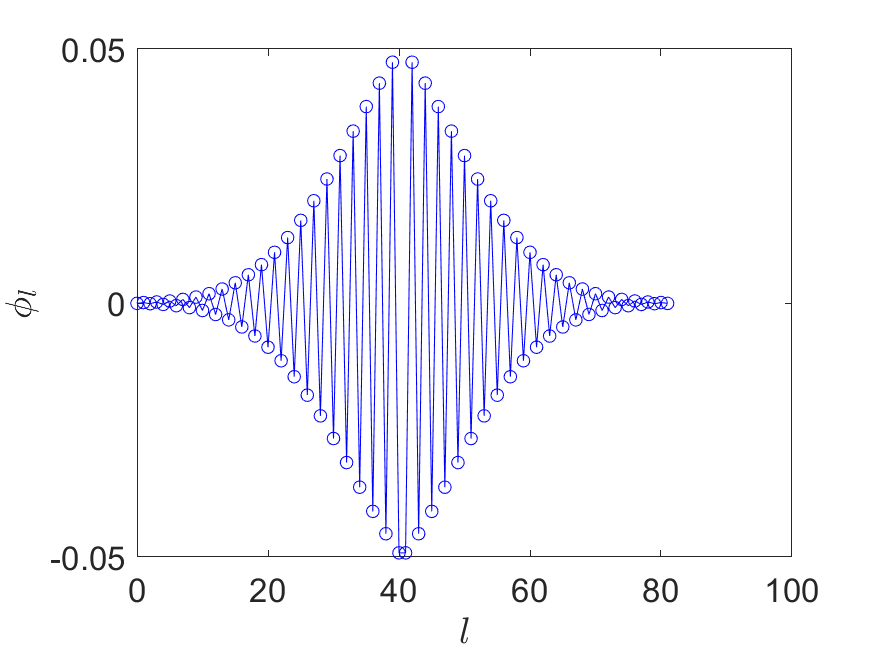
\includegraphics[width=0.31\textwidth]{inv_deg81_phase}
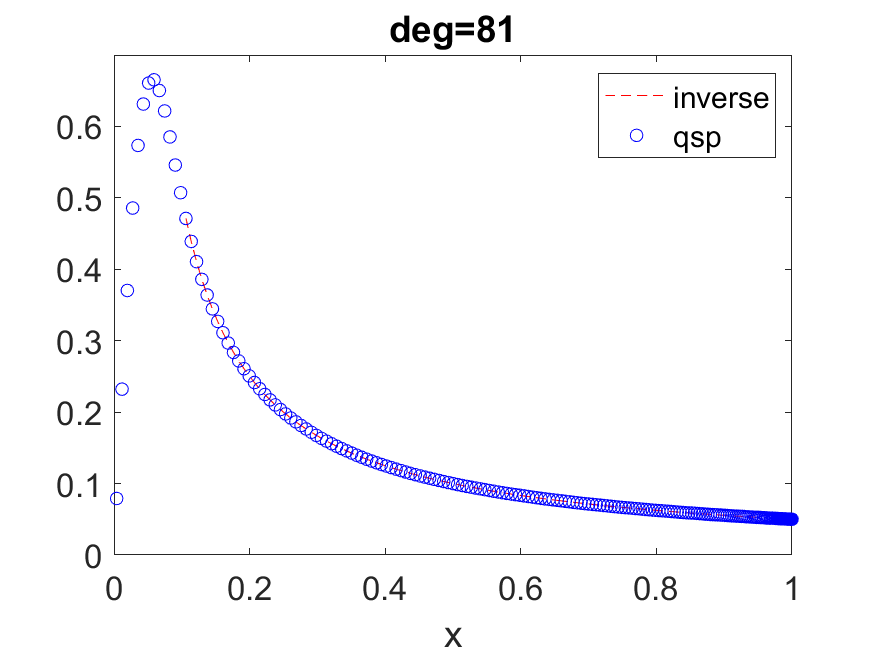
\includegraphics[width=0.31\textwidth]{inv_deg81_func}
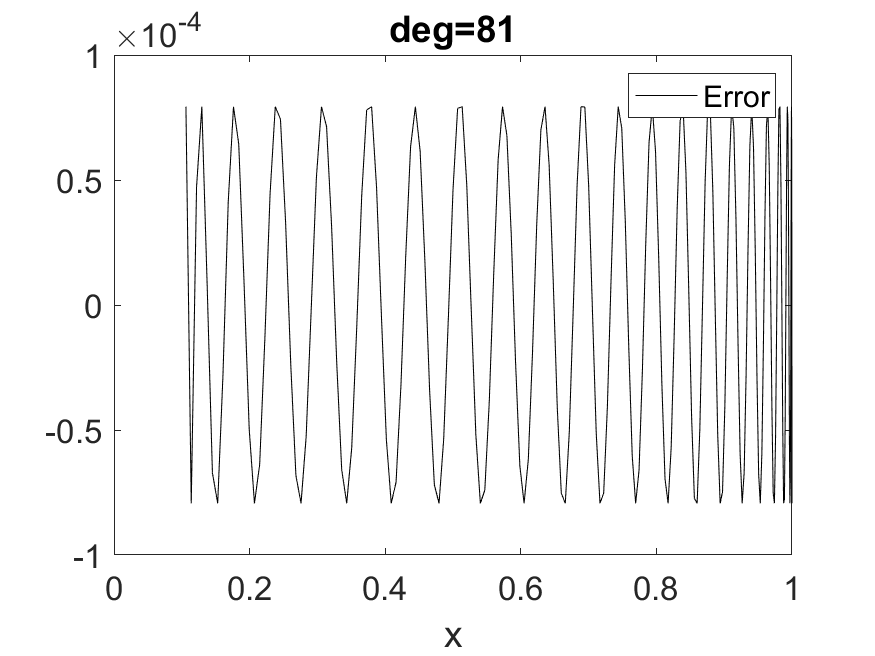
\includegraphics[width=0.31\textwidth]{inv_deg81_diff}
\end{center}
\caption{QSP representation of an odd polynomial approximating the inverse function on $[\kappa^{-1},1]$ with $\kappa=10$. The phase factors plotted removes a factor of $\pi/4$ on both ends (see \cref{eqn:phi0}).}
\label{fig:qsp_inv_deg81}
\end{figure}
 

Then \cref{fig:qsvt_circuit_real} implements a $(1,m+1)$-block-encoding of $p^{\diamond}(A^\dagger)=V p(\Sigma)W^\dagger$ denoted by $U_{\Phi}$. We have
\begin{equation}
\label{eq:block_encoding_err_A_inv}
    \|(p^{\diamond}(A^\dagger)-(\delta/\beta)A^{-1}\|=\|p(\Sigma)-(\delta/\beta)\Sigma^{-1}\|\leq \epsilon'.
\end{equation}
The total number of queries to to $U_A$ and $U_A^{\dag}$ is
\begin{equation}
\Or\left(\frac{1}{\delta}\log\left(\frac{1}{\epsilon'}\right)\right)
=\Or\left(\kappa\log\left(\frac{1}{\epsilon'}\right)\right).
\end{equation}

To solve QLSP, we assume the right hand side vector $\ket{b}$ can be accessed through the oracle $U_b$ such that
\begin{equation}
U_b\ket{0^n}=\ket{b}.
\end{equation}
We introduce the parameter 
\begin{equation}
\xi=\norm{A^{-1}\ket{b}},
\end{equation}
which plays an important part in the success probability of the procedure. Let 
\begin{equation}
x=(\delta/\beta)A^{-1}\ket{b}
\end{equation}
be the unnormalized true solution, and the normalized solution state is  $\ket{x}=x/\norm{x}$.
Now denote $\wt{x}=p^{\diamond}(A^{\dagger})\ket{b}$, and $\ket{\wt{x}}=\wt{x}/\norm{\wt{x}}$. Then the unnormalized solution satisfies $\|x-\wt{x}\|\leq\epsilon'$. 
For the normalized state $\ket{y}$, this error is scaled accordingly. When $\epsilon'\ll \|\ket{\wt{x}}\|$, we have
\begin{equation}
\|\ket{x}-\ket{x}\|\approx \frac{\|\wt{x}-x\|}{\|\wt{x}\|}\leq \frac{\epsilon'}{\|\wt{x}\|}.
\end{equation}
Also we have
\begin{equation}
\|\wt{x}\| = \left\|\frac{\delta}{\beta}A^{-1}\ket{b}\right\| = \frac{\delta\xi}{\beta} = \frac{\xi}{\beta\kappa}.
\end{equation}
Therefore in order for the normalized output quantum state to be $\epsilon$-close to the normalized solution state $\ket{x}$, we need to set $\epsilon'=\Or(\epsilon  \xi /\kappa)$.
This is similar to the case of the HHL algorithm in \cref{sec:HHL}, where QPE needs to achieve $\epsilon$ multiplicative accuracy, which means that the additive accuracy parameter $\epsilon'$ should be set to $\Or(\epsilon/\kappa)$.

The success probability of the above procedure is $\Omega(\|\wt{x}\|^2)=\Omega(\xi^2/\kappa^2)$. With amplitude amplification we can boost the success probability to be greater than $1/2$ with one qubit serving as a witness, i.e., if measuring this qubit we get an outcome 0 it means the procedure has succeeded, and if 1 it  means the procedure has failed. 
It takes $\Or(\kappa/\xi)$ rounds of amplitude amplification, i.e., using $U_{\Phi}^\dagger$, $U_{\Phi}$, $U_b$, and $U_b^\dagger$ for $\Or(\kappa/\xi)$ times.
A single $U_{\Phi}$ uses $U_A$ and its inverse
\begin{equation}
\Or\left(\frac{1}{\delta}\log\left(\frac{1}{\epsilon'}\right)\right)
=\Or\left(\kappa\log\left(\frac{\kappa}{\epsilon\xi}\right)\right)
\end{equation}
times.
Therefore the total number of queries to $U_A$ and its inverse is 
\begin{equation}
\Or\left(\frac{\kappa^2}{\xi} \log\left(\frac{\kappa}{\xi\epsilon}\right)\right).
\end{equation}
The number of queries to the $U_b$ and its inverse is $\Or(\kappa/\xi)$. 
We consider the following two cases for the magnitude of $\xi$. 
\begin{enumerate}\label{enum:two_cases}
    \item  In general if no further promise is given, then $\xi\geq 1$. The total query complexity of $U_A$ is therefore $\Or(\kappa^2 \log(\kappa/\epsilon))$. This is the typical complexity referred to in the literature.
    \item If $\ket{b}$ has a $\Omega(1)$ overlap with the left-singular vector of $A$ with the smallest singular value, then $\xi=\Omega(\kappa)$. This is the best case scenario, and the total query complexity of $U_A$ is  $\Or(\kappa \log(1/\epsilon))$, and the number of queries to the right hand side vector $\ket{b}$ is $\Or(1)$, which is independent of the condition number. 
\end{enumerate} 



\section{Quantum singular value transformation with basis transformation*}

So far we have assumed that we have a matrix $A$ in mind, and the access to $A$ is provided via the block encoding matrix $U_A$.
The QSVT circuit takes the form
\begin{equation}
U_{\Phi}= \opr{CR}_{\wt{\phi}_{0}}\cdots \opr{CR}_{\wt{\phi}_{d-2}}U_A^{\dag}\opr{CR}_{\wt{\phi}_{d-1}}U_A \opr{CR}_{\wt{\phi}_d}.
\end{equation}
If we are further given two unitary matrices $P,Q$, we can equivalently rewrite the QSVT transformation as
\begin{equation}
U_{\Phi}= \cdots (Q^{\dag}U_A^{\dag}P)^{\dag}(Q\opr{CR}_{\wt{\phi}_{d-1}}Q^{\dag})(QU_A P^{\dag})(P\opr{CR}_{\wt{\phi}_d}P^{\dag})P.
\end{equation}
The beginning of the equation ends with $P$ or $Q$ depending on the parity of $d$. The insertion of $P,Q$ amounts to a \textit{basis transformation}. Assume that we have access to $\wt{U}_A=QU_A P^{\dag}$, 
then $U_A$ is the matrix representation of $\wt{U}_A$ with respect to the bases given by $P,Q$, respectively.
What is different is that the controlled rotations before $U_A$ and $U_A^{\dag}$ are now expressed with respect to two different basis sets, i.e., $P\opr{CR}_{\wt{\phi}_d}P^{\dag}$, and $Q\opr{CR}_{\wt{\phi}_{d-1}}Q^{\dag}$, respectively. 
This can be useful for certain applications. 
Let us now express these ideas more formally.

Assume that we are given an $(n+m)$-qubit unitary $\wt{U}_A$, and two $(n+m)$-qubit projectors $\Pi,\Pi'$.  
For simplicity we assume $\opr{rank}(\Pi)=\opr{rank}(\Pi')=N$. 
Define an orthonormal basis set
\begin{equation}
\mc{B}=\{\ket{\varphi_0},\ldots,\ket{\varphi_{N-1}},\ket{v_N},\ldots,\ket{v_{NM-1}}\},
\label{eqn:qsvt_proj_basis_b}
\end{equation}
where the vectors $\ket{\varphi_0},\ldots,\ket{\varphi_{N-1}}$ span the range of $\Pi$, and all states $\ket{v_i}$ are orthogonal to $\ket{\varphi_j}$.
Similarly define an orthonormal basis set
\begin{equation}
\mc{B}'=\{\ket{\psi_0},\ldots,\ket{\psi_{N-1}},\ket{w_N},\ldots,\ket{w_{NM-1}}\}
\label{eqn:qsvt_proj_basis_bp}
\end{equation}
where the vectors $\ket{\psi_0},\ldots,\ket{\psi_{N-1}}$ span the range of $\Pi'$, and all states $\ket{w_i}$ are orthogonal to $\ket{\psi_j}$.
We can think that the columns of $\mc{B},\mc{B}'$ form the basis transformation matrix $P,Q$, respectively.

Then the matrix $A$ is defined implicitly in terms of its matrix representation
\begin{equation}
[\wt{U}_A]_{\mc{B}}^{\mc{B}'}=U_A=\begin{pmatrix}
A & * \\
* & *
\end{pmatrix}.
\label{eqn:qsvt_proj_blockencode}
\end{equation}
Note that 
\begin{equation}
[\Pi]_{\mc{B}}^{\mc{B}}=[\Pi']_{\mc{B'}}^{\mc{B'}}=\begin{pmatrix}
I_n & 0 \\
0 & 0
\end{pmatrix}=\ket{0^m}\bra{0^m}\otimes I_n,
\end{equation}
we find that 
\begin{equation}
\Pi'\wt{U}_A\Pi=\sum_{i,j\in [N]}\ket{\psi_i} A_{ij}\bra{\varphi_j}.
\end{equation}
Therefore \cref{thm:qsvt_real} can be viewed as the singular value transformation of $A$, which is a submatrix of the \emph{matrix representation} of $U_A$ with respect to bases $\mc{B},\mc{B}'$. 

The implementation of the controlled rotation $P\opr{CR}_{\wt{\phi}}P^{\dag}$ relies on the implementation of $\opr{C}_{\Pi}\opr{NOT}$.
The projectors $\Pi,\Pi'$ can be accessed directly, and WLOG we focus on one projector $\Pi$. 
Motivated from Grover's search, we may assume access to a reflection operator
\begin{equation}
R_{\Pi}=I_m-2\Pi.
\end{equation}
via the controlled NOT gates $\opr{C}_{\Pi}\opr{NOT},\opr{C}_{\Pi'}\opr{NOT}$ respectively. We can then define an $m$-qubit controlled NOT gate as
\begin{equation}
\opr{C}_{\Pi}\opr{NOT}:=X\otimes \Pi+I\otimes (I_{m}-\Pi),
\end{equation}
which can be constructed using $R_{\Pi}$ as
\begin{equation}
\begin{split}
\opr{C}_{\Pi}\opr{NOT}&=X\otimes \frac{I_m-R_{\Pi}}{2}+I\otimes \frac{I_m+R_{\Pi}}{2}\\
&=\frac{I+X}{2} \otimes I_m + \frac{I-X}{2} \otimes R_{\Pi}\\
&=\ket{+}\bra{+}\otimes I_m+\ket{-}\bra{-}\otimes R_\Pi\\
&=(H\otimes I_m)(\ket{0}\bra{0}\otimes I_m+\ket{1}\bra{1}\otimes R_\Pi)(H\otimes I_m).
\end{split}
\label{eqn:reflection_cpinot}
\end{equation}
Therefore assuming access to $R_{\Pi}$, the $\opr{C}_{\Pi}\opr{NOT}$ gate can be implemented using the circuit in \cref{fig:implement_CPINOT}.

\begin{figure}[H]
\begin{center}
\begin{quantikz}
\qw&\gate{H}& \ctrl{1}\qw& \gate{H}&\qw\\
\qw&\qw& \gate{R_{\Pi}}& \qw&\qw\\
\end{quantikz}
\end{center}
\caption{Circuit for implementing $\opr{C}_{\Pi}\opr{NOT}$ using a reflector $R_{\Pi}$.}
\label{fig:implement_CPINOT}
\end{figure}


Then according to \cref{thm:qsvt_real}, we can implement the QSVT using $\wt{U}_A,\wt{U}_A^{\dag}$, $\opr{C}_{\ket{0^m}\bra{0^m}}\opr{NOT}$ and single qubit rotation gates, where $\ket{0^m}\bra{0^m}\otimes I_n$ is a rank-$2^n$ projector. In this generalized setting, $\opr{C}_{\ket{0^m}\bra{0^m}\otimes I_n}\opr{NOT}=\opr{C}_{\ket{0^m}\bra{0^m}}\opr{NOT}\otimes I_n$ in the $\mc{B},\mc{B}'$ basis should be implemented using $\opr{C}_{\Pi}\opr{NOT},\opr{C}_{\Pi'}\opr{NOT}$, respectively.
We arrive at the following theorem:
\begin{thm}[Quantum singular value transformation with real polynomials and projectors]
Let $\wt{U}_A$ be a $(n+m)$-qubit unitary, and $\Pi,\Pi'$ be two $(n+m)$-qubit projectors of rank $2^n$.
Define the basis $\mc{B},\mc{B'}$ according to \cref{eqn:qsvt_proj_basis_b,eqn:qsvt_proj_basis_bp}, and let $A\in\CC^{N\times N}$ be defined in terms of the matrix representation in \cref{eqn:qsvt_proj_blockencode}. 
Given a polynomial $P_{\Re}(x)\in\RR[x]$ of degree $d$ satisfying the conditions in \cref{thm:qsp_real}, we can find a sequence of phase factors $\Phi\in\RR^{d+1}$ to define a unitary $U_{\Phi}$ satisfying
\begin{equation}
U_{\Phi}\ket{\varphi_j}=\sum_{i\in[N]}\ket{\psi_i} [P^{\diamond}_{\Re}(A)]_{ij}+\ket{\perp_j'},
\end{equation}
if $d$ is odd, and 
\begin{equation}
U_{\Phi}\ket{\varphi_j}=\sum_{i\in[N]}\ket{\varphi_i} [P^{\triangleright}_{\Re}(A)]_{ij}+\ket{\perp_j}.
\end{equation}
if $d$ is even. 
Here  $\Pi'\ket{\perp_j'}=0$, $\Pi\ket{\perp_j}=0$, and
$U_{\Phi}$ uses $\wt{U}_A,\wt{U}_A^{\dag}$, $\opr{C}_{\Pi}\opr{NOT},\opr{C}_{\Pi'}\opr{NOT}$, and single qubit rotation gates for $\Or(d)$ times.
\label{thm:qsvt_real_proj}
\end{thm}





\section{Application: Grover's search revisited, and fixed-point amplitude amplification*}\label{sec:appqsvt_grover}

As an application, let us revisit the Grover search problem from the perspective of QSVT.
Again let $\ket{x_0}$ be the desired marked state, and $\ket{\psi_0}$ be the uniform superposition of states.
Now let us perform a basis transformation. 
We define an orthonormal basis set $\mc{B}=\{\ket{\psi_0},\ket{v_1},\ldots,\ket{v_{N-1}}\}$, where all states $\ket{v_i}$ are orthogonal to $\ket{\psi_0}$. 
Similarly define an orthonormal basis set $\mc{B}'=\{\ket{x_0},\ket{w_1},\ldots,\ket{w_{N-1}}\}$, where all states $\ket{w_i}$ are orthogonal to $\ket{x_0}$.
Then the matrix of reflection operator $R_{\psi_0}$ with respect to $\mc{B},\mc{B'}$ is (let $a=1/\sqrt{N}$)
\begin{equation}
[R_{\psi_0}]_{\mc{B}}^{\mc{B}'}=\begin{pmatrix}
a & *\\
* & *
\end{pmatrix},
\end{equation}
Let $A=a$ be a $1\times 1$ matrix, and then $R_{\psi_0}\in \BE_{1,n}(A)$.
Furthermore, the projectors $\Pi=\ket{\psi_0}\bra{\psi_0}$ and $\Pi'=\ket{x_0}\bra{x_0}$ can be accessed via the reflection operator $R_{\psi_0},R_{x_0}$, respectively.
According to \cref{eqn:reflection_cpinot}, this defines $\opr{C}_{\Pi}\opr{NOT},\opr{C}_{\Pi'}\opr{NOT}$.
Let $\wt{U}_A=R_{\psi_0}$, we have
\begin{equation}
\Pi' \wt{U}_A\Pi=a\ket{x_0}\bra{\psi_0},
\end{equation}
and we would like to use \cref{thm:qsvt_real_proj} to find $U_{\Phi}$ that block encodes
\begin{equation}
\ket{x_0}P_{\Re}^{\diamond}(a)\bra{\psi_0}\approx \ket{x_0}\bra{\psi_0}.
\end{equation}
To this end, we need to find an \emph{odd}, real polynomial $P_{\Re}(x)$ satisfying $P_{\Re}(a)\approx 1$.
More specifically, we need to find $P_{\Re}(x)$ satisfying
\begin{equation}
\abs{P_{\Re}(x)-1}\le \epsilon^2, \quad \forall x\in [a,1].
\end{equation}
We can achieve this by approximating the sign function, with $\deg(P_{\Re})=\Or(\log(1/\epsilon^2) a^{-1})=\Or(\log(1/\epsilon)\sqrt{N})$ (see e.g.~\cite[Corollary 6]{LowChuang2017a}). 
This construction is also based on an approximation to the $\mathrm{erf}$ function.
\cref{fig:qsp_sign_deg81} gives a concrete construction of an odd polynomial obtained via numerical optimization, and the phase factors are obtained via QSPPACK.


\begin{figure}[H]
\begin{center}
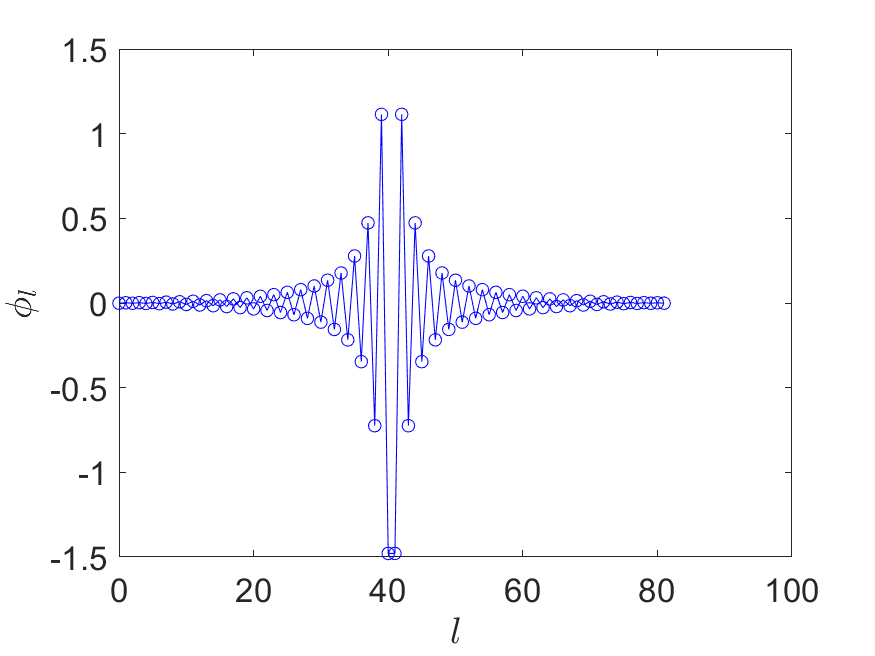
\includegraphics[width=0.31\textwidth]{sign_deg81_phase}
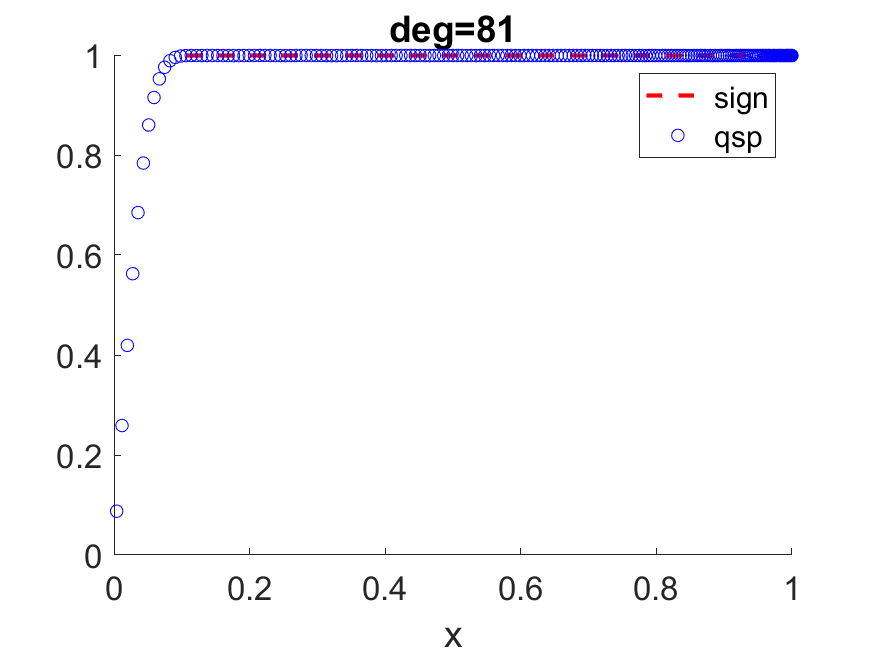
\includegraphics[width=0.31\textwidth]{sign_deg81_func}
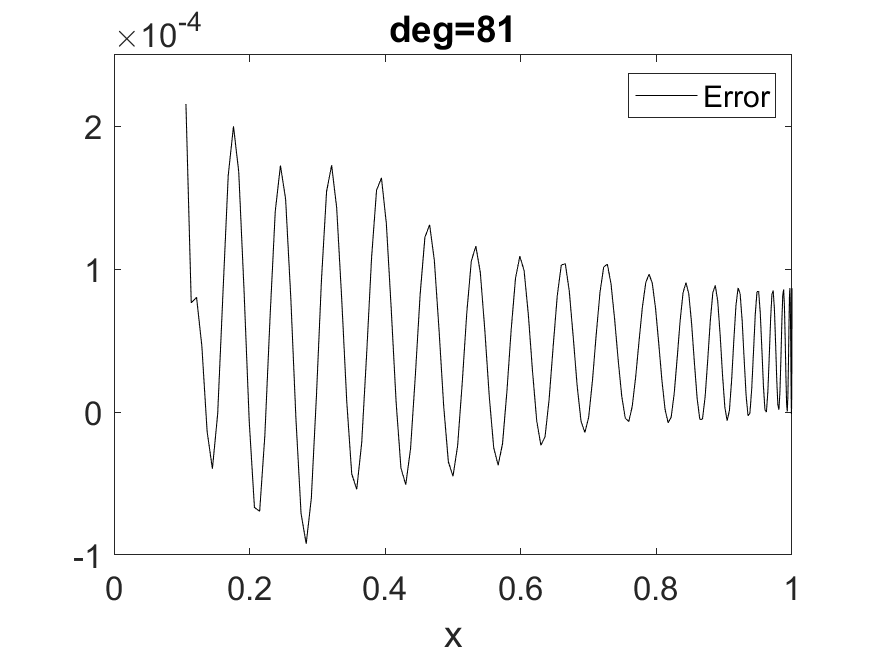
\includegraphics[width=0.31\textwidth]{sign_deg81_diff}
\end{center}
\caption{QSP representation of an odd polynomial approximating the sign function on $[0.1,1]$. The phase factors plotted removes a factor of $\pi/4$ on both ends (see \cref{eqn:phi0}).}
\label{fig:qsp_sign_deg81}
\end{figure}
 



Then
\begin{equation}
U_{\Phi}\ket{\psi_0}\approx \ket{x_0}.
\end{equation}
More specifically, note that
\begin{equation}
U_{\Phi}\ket{\psi_0} - \ket{x_0}=(P_{\Re}(a)-1)\ket{\psi_0}+\ket{\wt{\perp}}
\end{equation}
for some unnormalized state $\ket{\wt{\perp}}$. Moreover
\begin{equation}
\norm{\ket{\wt{\perp}}}^2+P_{\Re}^2(a)=1,
\end{equation}
which gives
\begin{equation}
\norm{\ket{\wt{\perp}}}= \sqrt{1-P_{\Re}^2(a)}\le \sqrt{1-(1-\epsilon^{2})^2}\le \sqrt{2\epsilon^2}.
\end{equation}
So 
\begin{equation}
\norm{U_{\Phi}\ket{\psi_0} - \ket{x_0}}\le \epsilon^2+\sqrt{2}\epsilon=\Or(\epsilon).
\end{equation}
Therefore we can measure the system register to find $x_0$, and we achieve the same Grover type speedup.

Note that the approximation can be arbitrarily accurate, and there is no overshooting problem (though this is a small problem) as in the standard Grover search. 
While Grover's search does not require the output quantum state to be exactly $\ket{x_0}$, this could be desirable when it is used as a quantum subroutine, such as amplitude amplification.

The immediate generalization of the procedure above is called the fixed point amplitude amplification. 

\begin{prop}[Fixed-point amplitude amplification]
Let $\wt{U}_A$ be an $n$-qubit unitary and $\Pi'$ be an $n$-qubit orthogonal projector such that 
\begin{equation}
\Pi' \wt{U}_A\ket{\varphi_0}=a\ket{\psi}, \quad a> \delta>0.
\end{equation}
Then there is a $(n+1)$-qubit unitary circuit $U_{\Phi}$ such that
\begin{equation}
\norm{\ket{0}\ket{\psi}-U_{\Phi}\ket{0}\ket{\varphi_0}}\le \epsilon.
\end{equation}
here $U_{\Phi}$ uses the gates $\wt{U}_A,\wt{U}_A^{\dag},\opr{C}_{\Pi'}\opr{NOT},\opr{C}_{\ket{\varphi_0}\bra{\varphi_0}}\opr{NOT}$ and single qubit rotation gates for $\Or(\log(1/\epsilon) \delta^{-1})$ times.
\label{prop:fixedpt_aa}
\end{prop}
\begin{proof}
The procedure is very similar to Grover's search.
We only prove the case when $\Pi$ is of rank $1$, though the statement is also correct when the rank of $\Pi$ is larger than $1$.
We can construct $\mc{B}=\{\ket{\varphi_0},\ket{v_1},\ldots,\ket{v_{N-1}}\}$, where all states $\ket{v_i}$ are orthogonal to $\ket{\varphi_0}$. 
Similarly define an orthonormal basis set $\mc{B}'=\{\ket{\psi},\ket{w_1},\ldots,\ket{w_{N-1}}\}$, where all states $\ket{w_i}$ are orthogonal to the target state $\ket{\psi}$.
Since the target state $\ket{\psi}$ belongs to the range of $\Pi'$, 
\begin{equation}
\braket{\psi|\wt{U}_A|\varphi_0}=\braket{\psi|\Pi '\wt{U}_A|\varphi_0}=a,
\end{equation}
i.e.,
\begin{equation}
[\wt{U}_A]_{\mc{B}}^{\mc{B}'}=\begin{pmatrix}
a & *\\
* & *
\end{pmatrix}.
\end{equation}
 Now let $\Pi=\ket{\varphi_0}\bra{\varphi_0}$, we can use the same choice of $P_{\Re}(x)$ as in Grover's search so that $\abs{P_{\Re}(x)-1}=\Or(\epsilon^2)$ for any $x\ge \delta$, and $\deg(P_{\Re})=\Or(\log(1/\epsilon) \delta^{-1})$.
The corresponding $U_{\Phi}$ uses one ancilla qubit to block encode
\begin{equation}
\ket{\psi} P_{\Re}(\delta)\bra{\varphi_0}\approx \ket{\psi} \bra{\varphi_0}.
\end{equation} 
 \end{proof}

Note that the ranks of $\Pi',\Pi$ are different. This does not affect the proof. 


\vspace{2em}

\begin{exer}[Robust oblivious amplitude amplification]
Consider a quantum circuit consisting of two registers denoted by $a$ and $s$. Suppose we have a block encoding $V$ of $A$: $A=(\bra{0}_a\otimes I_s)V(\ket{0}_a\otimes I_s)$. Let $W=-V(\mathrm{REF}\otimes I_s)V^{\dagger}(\mathrm{REF}\otimes I_s)V$, where $\mathrm{REF}=I_a-2\ket{0}_a\bra{0}_a$. (1) Within the framework of QSVT, what is the polynomial associated with the singular value transformation implemented by $W$? (2) Suppose $A=U/2$ for some unitary $U$. What is $(\bra{0}_a\otimes I_s)W(\ket{0}_a\otimes I_s)$? (3) Explain the construction of $W$ in terms of a singular value transformation $f^{\diamond}(A)$ with $f(x)=3x-4x^3$. Draw the picture of $f(x)$ and mark its values at $x=0,\frac12,1$.
\end{exer}

\begin{exer}[Logarithm of unitaries]
  Given access to a unitary $U=e^{\I H}$ where $\norm{H}\le \pi/2$. Use QSVT to design a quantum algorithm to approximately implement a block encoding of $H$, using controlled $U$ and its inverses, as well as elementary quantum gates.
\end{exer}
